%
% $Id: ch04_implementation.tex
%
%   *******************************************************************
%   * SEE THE MAIN FILE "AllegThesis.tex" FOR MORE INFORMATION.       *
%   *******************************************************************
%
\chapter{Implementation}\label{ch:implem}
This chapter outlines the design of the project. The packages and resources outlined
in the previous chapter are referenced in how they were used in the project design.
Many of the methods from the source code are outlined and explained, in order of how
they may be accessed by a user.

\section{Main Menu}
Due to time constraints of the thesis, much of this project still currently exists
as \textit{Python} scripts, which execute in the terminal. As such, to start the
project, the user must execute in the terminal.
\begin{lstlisting}[language=bash]
  $ python3 main.py
\end{lstlisting}

The \textit{main.py} serves only as a gateway to the two current scripts,
\textit{recent.py} and \textit{edit.py}. The available input options are "recent",
"edit", and "exit". The entire script is encompassed in a while loop, such that
an incorrect input simply prompt the user for another input. The function scripts
are called using: \begin{verbatim} exec(open("./file.py").read()) \end{verbatim}

\section{Playlist Editor}
\textit{edit.py} is used to edit a user's existing playlists by filtering them
using the Spotipy API data. As outlined in the previous chapter, this project uses
the Spotipy wrapper for the official API, written in JavaScript. The constructor
function (Figure 4.1) is used for user authentication; the \texttt{CLIENT\_ID},
\texttt{CLIENT\_SECRET}, \texttt{REDIRECT\_URI},
and SCOPE variables are all needed for any projects that use the Spotify API.

\pagebreak
\begin{figure}
\begin{lstlisting}[aboveskip=0pt]
  def __init__(self):
    self.CLIENT_ID = SPOTIPY_CLIENT_ID
    self.CLIENT_SECRET = SPOTIPY_CLIENT_SECRET
    self.REDIRECT_URI = "http://localhost:5000"
    self.SCOPE = "playlist-read-private playlist-modify-private
    playlist-read-collaborative
    playlist-modify-public"
    self.sp = self.getUser() #Creates Spotify instance
    self.id = self.sp.me()["id"] #Gets ID of authenticating user
\end{lstlisting}
\caption{{\tt edit.py} constructor}
\end{figure}

Once the user is authenticated, the \textit{getPlaylist} function (Figure 4.2) gets the name
of every playlist the user has created or followed on Spotify. It also assigns
a numeric value to each one.


\begin{figure}
\begin{lstlisting}[aboveskip=5pt]
  def getPlaylist(self):
    #This function gets all playlists from the user.
    results = self.sp.current_user_playlists()
    for i, item in enumerate(results["items"]):
      print ("{number} {name}".format(number=i, name=item["name"]))
\end{lstlisting}
\caption{{\tt edit.py getPlaylist} function}
\end{figure}

The user then inputs the corresponding number to the playlist they desire to
filter. On the selection, a series of graphs are generated, illustrating the
distribution of the editable end points of songs in the playlist. When the user
closes these plots, they are prompted to enter the low and high values of the
end points of the tracks, in the \textit{getLimits} function. Leaving the input
empty will automatically choose the lowest and highest possible values for each
set, so if a certain criteria doesn't matter, no songs will be excluded by it.

The \textit{getSongs} function is then triggered, which
returns the song IDs for every track in the playlist. Once the track IDs are
gathered, the song features are returned using the \textit{getFeatures} function.
Thanks to Spotipy, this takes only a single line of code. (Figure 4.3)

\begin{figure}[!h]
\begin{lstlisting}
def getFeatures(self, track):
  #This function retrieves audio features from Spotify
  features = self.sp.audio_features(track)
  return features
\end{lstlisting}
\caption{{\tt edit.py getFeatures} function}
\end{figure}

It is at this point that the API end points are utilized, in the \textit{sortSongs}
function. In a series of nested \textit{if} statements, each desired range is
checked for each value of the songs. If they all return true, the song "passes",
and is added to the generated playlist. The \textit{createPlaylist} function
takes the passing songs, and creates a playlist using two Spotipy methods:
\textit{user\_playlist\_create} and \textit{user\_playlist\_add\_tracks}.
At this point, plots with an identical format as generated from the initial playlist
are once again created, in order to concretely visualize the new changes. The final
line to execute opens the user's playlists in a web page, using the \textit{open\_new\_tab}
method from the \textit{webbrowser} package. This puts the user one click away from
the newly generated playlist.

\section{Web Interface}
The \textit{recent.py} file is a venture into creating a web portal, using the Flask
framework to facilitate the use of \textit{Python}, as outlined in the previous
chapter. Initialized similarly to \textit{edit.py}, the authorization process
is nearly identical, but with more robustness. Upon either creation or discovery
of the authentication token, the Flask app will first return the last 50 tracks
the user has saved to their profile, using the \textit{current\_user\_saved\_tracks}
method. Unfortunately, the Spotify API limits rates to 50 per call, but an if statement
paired with a dynamic offset in the \textit{getSongList} function allows this
number to be increased, albeit with a very miniscule cooldown time.

\begin{figure}[!h]
\begin{lstlisting}
if callNo == 0:
        offset = 0
    else:
        offset = callNo*min(playlistLength, 50)

    results = sp.current_user_saved_tracks(limit=min(playlistLength, 50), offset=offset)
\end{lstlisting}
\caption{Dynamic Offset}
\end{figure}


The app then opens an HTML template. The user is
presented with a form, in which they may choose to create a Spotify playlist,
with options for the number of songs, a limit to the number of songs by a single
artist, and whether the playlist should be shuffled or not. (Figure 4.5)

\begin{figure}[!h]
\begin{lstlisting}
<div>
    <form action="/run" method="POST">
    Number of songs: <br>
    <input type="number" name="playlistLength" value="50" min=20>
    <br><br>
    Max songs per artist: <br>
    <input type="number" name="maxSongs" value="3" min=1>
    <br><br>
    <input type="checkbox" name="shuffle" value="True">Shuffle Songs?
    <br><br>
    <input type="submit" value="Create Playlist!" autofocus>
    </form>
</div>
\end{lstlisting}
\caption{{\tt runRecentlyadded.html} input form}
\end{figure}



These values are passed into a thread in the \textit{run} function, which then
loads the \textit{running.html} page.

\begin{figure}[!h]
\begin{lstlisting}
<div>
    <h3>Generating playlist. Please wait...</h3>
    <progress value= {{ progress }} max="100"></progress>
</div>
\end{lstlisting}
\caption{{\tt running.html} progress bar}
\end{figure}

The \textit{running.html} is mainly a placeholder, but does include a progress
bar corresponding to the creation of the playlist (Figure 4.6).

In order to limit the maximum number of songs from a single artist, the code needed
the ability to generate \textit{r} random, sorted integers from [0, n). This method
was taken from an example by Raymond Hettinger \cite{Hettinger:04} (Figure 4.7).

After removing the excess songs, the playlist is created and populated, using
a similar method to \textit{edit.py}. On generation of the playlist, the user
is redirected to the \textit{success.html} template, which has options to view
the created playlist on Spotify's web player, and to go back to the input form.


\begin{figure}[!h]
\begin{lstlisting}
def sample(n, r):
    #taken from http://code.activestate.com/recipes/272884-random-samples-without-replacement/
    #Generate r randomly chosen, sorted integers from [0,n)
    rand = random.random
    pop = n
    for samp in range(r, 0, -1):
        cumprob = 1.0
        x = rand()
        while x < cumprob:
            cumprob -= cumprob * samp / pop
            pop -= 1
        yield n-pop-1
\end{lstlisting}
\caption{Hettinger's random generator}
\end{figure}

\clearpage

\section{Result Testing}

In order to empirically check the effectiveness of the playlist editing, the
Matplotlib library for Python \cite{Matplotlib:19} was used to generate graphs
showing the values of the audio features, before and after the editing process.
In addition to this, the "pandas" library \cite{Pandas:19} was used to create a
dataframe with the track data.


\begin{figure}[!h]
\begin{lstlisting}
  ax1 = fig2.add_subplot(331)
  ax1.set_xlabel('Danceability')
  ax1.set_ylabel('Count')
  ax1.set_title('Danceability Distribution')
  pos_dance.hist(alpha= 0.5, bins=30)
  ax2 = fig2.add_subplot(331)
  neg_dance.hist(alpha= 0.5, bins=30)
\end{lstlisting}
\caption{Plot Template}
\end{figure}

As seen above, eight graphs are generated, one for each available end point. The
graphs show the distribution of the end point values, as well as the amount of
tracks that have each value.

\begin{center}
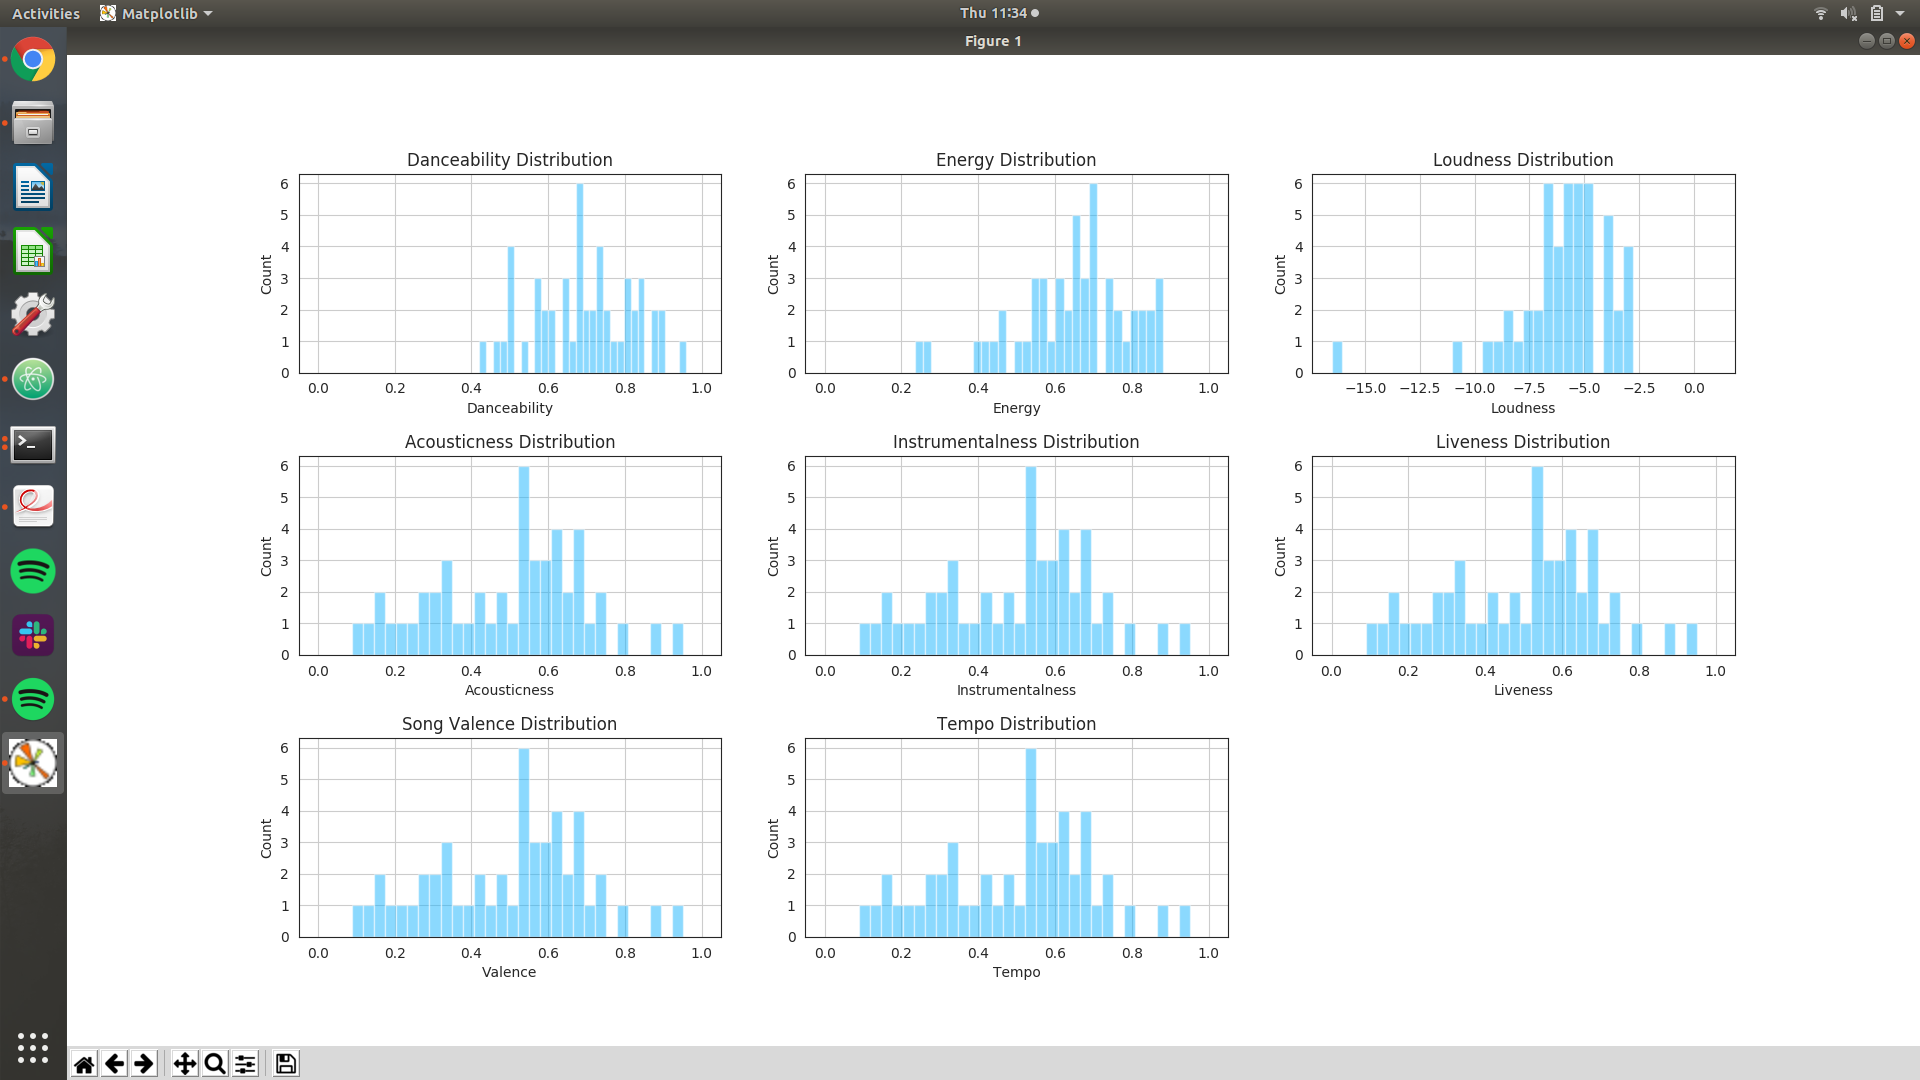
\includegraphics[height=8cm]{images/before.png}
\end{center}

The above graphs are generated from Spotify's "Today's Top Hits" playlist
\cite{Spotify:19}, which consists of the current 50 most popular songs in
Spotify's catalog. The values are reflective of current pop music, with a
heavy skew towards high energy music, which is also danceable. Interestingly,
valence is fairly evenly distributed, suggesting that some of the tracks subject
matters are sadder and more negative, but are still able to sound energetic
and danceable.

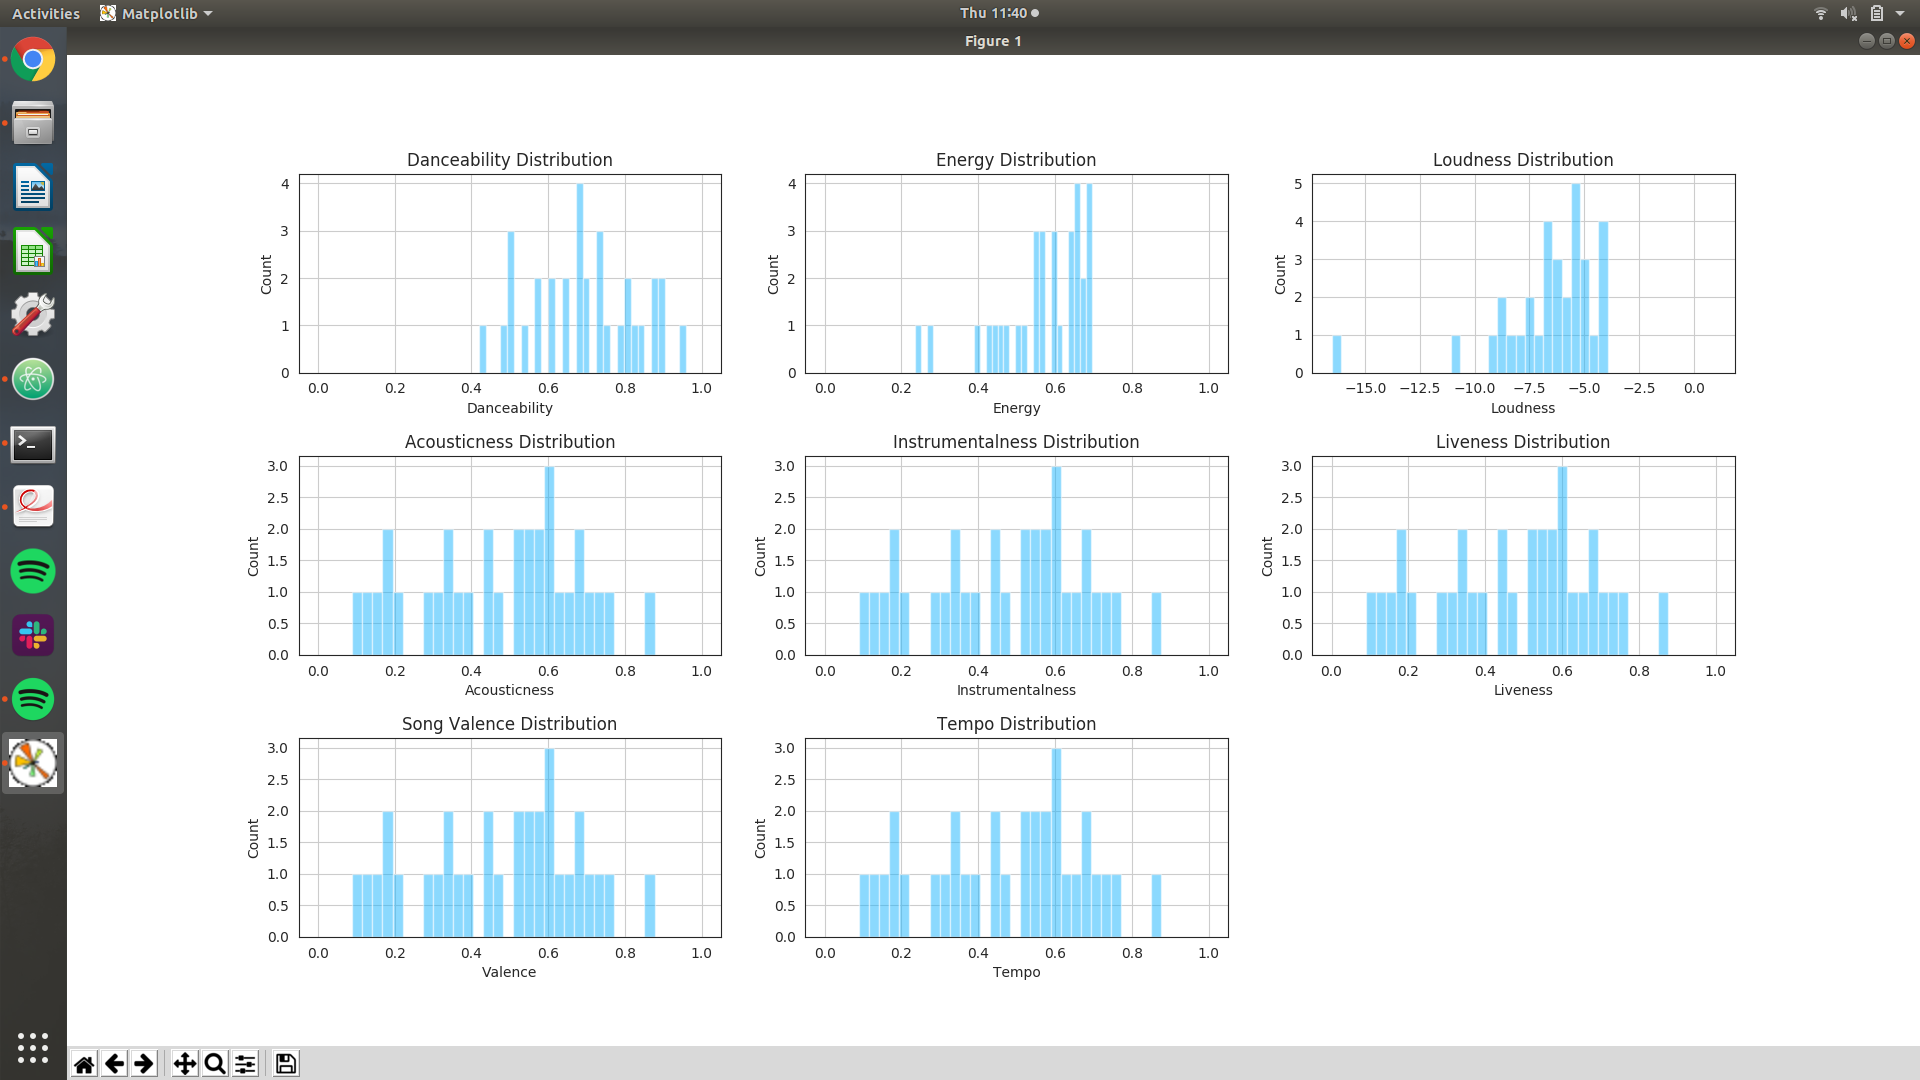
\includegraphics[height=8cm]{images/after.png}

These resulting graphs were aggregated from a playlist generated from "Today's Top Hits"
\cite{TopHits:19}, with the only applied requirement being energy less than 0.7.
Of course, the energy of the new playlist abruptly stops at .7, but the interesting
part is how several other end points are affected by this change. Loudness distribution
is limited to below -3.5 dB, which suggests that loudness is a major segment of the
formula used to calculate energy.

\section{Playlist Creation Efficiency}

\begin{figure}[!htb]
\begin{lstlisting}
if danceL <= songF["danceability"] <= danceH:
  if energyL <= songF["energy"] <= energyH:
    if loudL <= songF["loudness"] <= loudH:
      if acousticL <= songF["acousticness"] <= acousticH:
        if instrumentL <= songF["instrumentalness"] <= instrumentH:
          if livenessL <= songF["liveness"] <= livenessH:
            if valenceL <= songF["valence"] <= valenceH:
              if tempoL <= songF["tempo"] <= tempoH:
                return True
\end{lstlisting}
\caption{The sortSongs function}
\end{figure}

Due to the design of the function used to pick out songs that match the user
criteria, the playlist generation is the most time consuming element of the
program, most notably when applying to long playlists. Because of this, the
execution of each end point was measured, using the "time" Python library. This
was an attempt to see if the different endpoints took longer to sort than others,
and if the sorting process execution time was affected at all by the user defined
range of values. The Spotify-curated "Today's Top Hits" playlist \cite{TopHits:19}
was used to check each value. The first trials involved changing the ranges one
end point at a time, which resulted in a negligble amount of difference in
execution time for every variable. The next testing method was to attempt shrinking
the range of every variable simultaneously, compared to leaving every range
completely open. These changes also failed to create any noticeable difference
in execution time. This is likely due to the calls to the Spotify database,
which store the end points as identical types. Unless a more efficient way to
rewrite this method's code is found, the time to generate a playlist likely
will not be lowered. The execution time is limited by the necessary API calls,
which limits time optimization.

\section{Feasibility}
Due to the intrinsically subjective nature of music, graphical representations
which show that the playlist filtering is correctly working is not enough to
ensure that the resulting songs form an enjoyable listening experience. To this
end, the best testing method would involve human trials. Currently, I am the
only person to somewhat formally verify the correctness of the results, but
there are several avenues to allow more user feedback, which will likely be
pursued after the web portal is more complete. The first would be to simply
host the app on a web server, with a feedback form available for all users.
Questions relating to the user experience, and more specific inquiries about
satisfaction and accuracy of results would be valuable in tuning the metrics
for future use. Something as simple as a Google form could be used, with
questions including:
\begin{itemize}
  \item Did the application work correctly?
  \item Was the creator easy to use?
  \item How much, if any, music theory background do you have?
  \item Were you satisfied with the resulting songs?
  \item Were there any unwanted songs in the new playlist?
\end{itemize}
This feedback would be useful to gather another, outside perspective from my
own, hopefully making the project more accessible to any user.
Another available resource is the Spotify Developer Showcase
\cite{Spotify:19}, which features user developed projects built using the
Spotify API. Submitting Scottipy to the showcase would be another effective
way to increase the project's user base. These will be used after completing
the web portion of the project.
